\section{\'{E}cosyst\`{e}me du d\'{e}veloppeur}

\begin{frame}
    \begin{center}
    \fontsize{48pt}{7.2}\selectfont
    \'{E}cosyst\`{e}me du d\'{e}veloppeur
    \end{center}
\end{frame}

\subsection{Syst\`{e}me de gestion de version}
\begin{frame}
	\frametitle{SCM: Source Code Management}
    Qu\'{}ils soient centralis\'{e}s ou d\'{e}centralis\'{e}s, il existe plusieurs syst\`{e}mes (CSV, SVN, Mercurial, GIT, etc.).
    \\~\\
    Ces syst\`{e}mes fonctionnent par diff\'{e}rentiel (patch) afin de permettre de restaurer une version pr\'{e}c\'{e}dente ou encore de travailler sur une version parall\`{e}le qui pourra plus tard \^{e}tre r\'{e}-incorpor\'{e}e dans la version principale.
    \\~\\
    On parle de
    \begin{itemize}
      \item \textbf{branch} pour d\'{e}crire un fil de modification
      \item \textbf{tag} pour identifier une version bien particuli\`{e}re
      \item \textbf{merge}  lors de la r\'{e}union de deux branches
      \item \textbf{checkout} pour r\'{e}cup\'{e}rer la version d\'{}un d\'{e}p\^{o}t
      \item \textbf{commit} pour envoyer des modifications sur un d\'{e}p\^{o}t
    \end{itemize}
\end{frame}

\begin{frame}
	\frametitle{SCM: Source Code Management}
    ~\\
	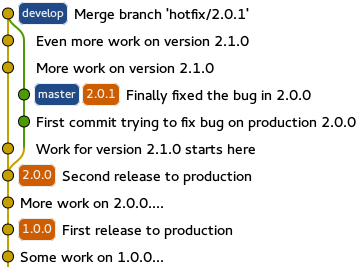
\includegraphics[width=8cm]{img/git_sample.png}
    ~\\
\end{frame}

\subsection{Moteur de construction}
\begin{frame}
	\frametitle{Build automation tool}
Du plus vieux (\textbf{make}) aux plus utilis\'{e}s dans le monde Java (\textbf{Maven}, \textbf{Graddle}), ces outils permettent de g\'{e}rer
~
\begin{itemize}
      \item les d\'{e}pendances utilis\'{e}es
      \item le lancement des tests
      \item la construction d'un projet (packaging)
      \item son rapport au syst\`{e}me de gestion de version
      \item son cycle de vie dans le syst\`{e}me d'int\'{e}gration continue
      \item son param\`{e}trage
      \item la g\'{e}n\'{e}ration de la documentation
    \end{itemize}
\end{frame}

\begin{frame}
	\frametitle{Maven I}
	\textbf{Maven} propose de baser l\'{}organisation du projet suivant des conventions plut\^{o}t que la description des t\^{a}ches n\'{e}cessaires \`{a} sa gestion.
	\\~\\
    Ainsi un projet \textbf{Maven} doit avoir cette structure
    \\
    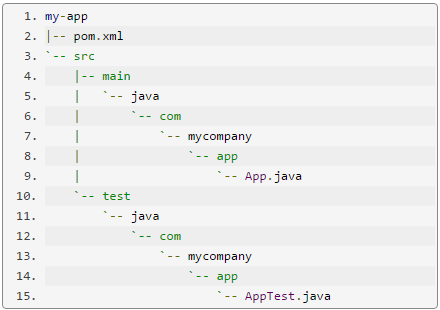
\includegraphics[width=7cm]{img/maven_structure.png}
\end{frame}

\begin{frame}
	\frametitle{Maven II}
    Par d\'{e}faut Maven utilise un cycle de vie permettant \`{a} la grande majorit\'{e} des projets d\'{}\^{e}tre construit sans configuration.
    \\~\\
    \url{https://maven.apache.org/guides/introduction/introduction-to-the-lifecycle.html}
    \\~\\
    Les principales \textbf{phases} sont
    \begin{itemize}
      \item \textbf{clean} : nettoie les fichiers compil\'{e}s ou g\'{e}n\'{e}r\'{e}s
      \item \textbf{compile} : compile les sources \textit{principales (main)}
      \item \textbf{test-compile} : compile les sources de \textit{test}
      \item \textbf{test} : lance les tests
      \item \textbf{package} : construit le binaire, \textbf{jar} par d\'{e}faut
      \item \textbf{install} : place le binaire dans le d\'{e}p\^{o}t Maven local
      \item \textbf{deploy} : place le binaire dans un d\'{e}p\^{o}t Maven distant
      \item \textbf{site} : g\'{e}n\'{e}re la documentation
    \end{itemize}
\end{frame}

\begin{frame}
	\frametitle{Maven III}
    Chaque phase est associable \`{a} un ou des \underline{\textbf{plugins}}, ce qui rend Maven tr\'{e}s extensible.
    \\~\\
    Des plugins sont fournis directement par Maven, comme le \textbf{maven-clean-plugin}.
    \\~\\
    D\'{}autre sont cr\'{e}\'{e}s par la communaut\'{e} sans voir besoin de modifier l\'{}outil :
    \begin{itemize}
      \item \textbf{cukedoctor-maven-plugin} : produit une version HTML du r\'{e}sultat des tests Cucumber
      \item \textbf{sonar-maven-plugin} : analyse le code avec diff\'{e}rents outils (PMD, Checkstyle, JaCoCo, etc.) et pousse les r\'{e}sultats dans un serveur Sonar
      \item etc.
    \end{itemize}
\end{frame}

\begin{frame}[fragile]
	\frametitle{Maven}
    \begin{center}
    \fontsize{48pt}{7.2}\selectfont
    D\'{e}mo
    \end{center}
    \begin{center}
    (Cr\'{e}ation d'un projet, g\'{e}n\'{e}ration de la documentation)
    \\~\\
    \begin{lstlisting}
mvn archetype:generate
	-DarchetypeArtifactId=maven-archetype-quickstart
    -DgroupId=fr.esiea
    -DartifactId=fruit-basket

mvn site
		\end{lstlisting} 
    \end{center}
\end{frame}

\begin{frame}
	\frametitle{Maven : phases \& plugins du packaging jar}
    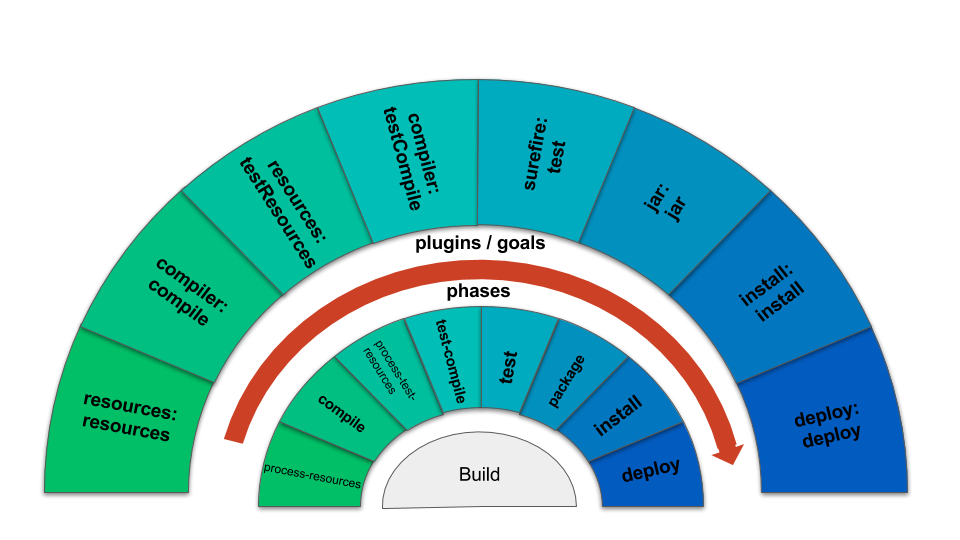
\includegraphics[width=11cm]{img/maven_circle.png}
\end{frame}

\subsection{D\'ep\^{o}t}
\begin{frame}
	\frametitle{Repository Manager}
    Il en existe plusieurs (Nexus, Artifactory, etc.) , c\'{}est l\'{}endroit o\`{u} vont tous les binaires.
    \\~\\
    Aussi bien ceux produits par l\'{}int\'{e}gration continue de votre projet que les d\'{e}pendances que votre projet utilise.
    \\~\\
    Pour cela, les diff\'{e}rents outils int\'{e}ragissant avec le d\'{e}p\^{o}t fonctionnent avec les conventions de nommage de Maven
    
\begin{itemize}
	\item Le \textbf{G.A.V} (\textbf{G}roupId, \textbf{A}rtifactId, \textbf{V}ersion) identifie un binaire
    \item La structure d'un d\'ep\^{o}t est identique \`{a} celle du d\'ep\^{o}t local
    \begin{itemize}
    	\item \textbf{\texttildelow{}/.m2/repository/}junit/junit/4.12/junit-4.12.jar
        \item \textbf{http://central.maven.org/maven2/}junit/junit/4.12/junit-4.12.jar
    \end{itemize}
\end{itemize}
\end{frame}

\subsection{IDE (Integrated development environment)}
\begin{frame}
	\frametitle{IDE}
    Il en existe plusieurs (Eclipse, IntelliJ, etc.), c\'{}est l\'{}outil qui aide le d\'{e}veloppeur \`{a} taper du code plus vite et en faisant moins d'erreur.
    \\~\\
    Pour cela, ces outils int\`{e}grent des raccourcis claviers aidant \`{a} la cr\'{e}ation rapide de fichier, de structure, au lancement de t\^{a}che r\'{e}p\'{e}titives, \`{a} la visualisation de la documentation.
    \\~\\
    Il est important pour un d\'{e}veloppeur d\'{}\^{e}tre \`{a} l'aise avec un IDE afin de produire rapidement des POC ou encore de s'attaquer \`{a} de gros \textit{refactoring} sans crainte d'erreur ou de r\'{e}gressions.
\end{frame}

\subsection{Plugins}
\begin{frame}
	\frametitle{Plugins}
    Un plugin (extension ou encore greffon) peut \^{e}tre vu comme l'inverse d'un framework en ce sens qu'un plugin va \^{e}tre appel\'{e} par du code et non le contraire.
    \\~\\
    La plupart des outils de d\'{e}veloppement offre une API permettant le d\'{e}veloppement de plugins.
    \\~\\
    C'est le cas de GIT, Maven, Eclipse, ou encore de Jenkins (int\'{e}gration continue).
    \\~\\
    \underline{Minimalistes} dans leurs concepts de base, ces outils autorisent \underline{l'ajout de} \underline{fonctionnalit\'{e}s}.
    \\~\\
    \textbf{L'ouverture \`{a} la composition} est un principe important de l'architecture logicielle ici mis en exemple.
\end{frame}

\subsection{Tests}
\begin{frame}
	\frametitle{Tests I}
    Les tests servent trois objectifs:
\begin{itemize}
    \item rassurer le d\'{e}veloppeur sur la bonne fonction de son code, maintenant et dans le futur
    \item rassurer l\'{}\'{e}quipe projet
    \item montrer comment le code produit doit ou peut \^{e}tre utilis\'{e}
\end{itemize}
~\\
On trouve commun\'{e}ment le d\'{e}coupage suivant:
\begin{itemize}
    \item Unit Test: teste un fragment de code, en g\'{e}n\'{e}ral une seule m\'{e}thode ($<$300ms)
    \item Integration Test: teste l'interfacage avec un framework, un autre applicatif, etc. ($<$1min)
    \item Acceptance Test: teste une fonctionnalit\'{e} compl\`{e}te du point de vue m\'{e}tier
\end{itemize}
\end{frame}

\begin{frame}
	\frametitle{Tests II}
    Chacun de ces types de test est int\'{e}ressant et se focalise sur des objectifs diff\'{e}rents.
    \\~\\
    Si des tests doivent \^{e}tre longs, il faut qu'ils soient pertinents.
    \\~\\
    De cette mani\`{e}re la boucle de r\'{e}tro-action est la plus courte possible.
    \\~\\
    Il est donc n\'{e}cessaire de mat\'{e}rialiser une diff\'{e}rence entre chaque type de test.
	\\~\\
	Maven propose une convention : *Test.java et *IT.java
    \\~\\
    Configuration par d\'{e}faut des plugins \textbf{maven-surefire-plugin} et \textbf{maven-failsafe-plugin} li\'{e}s aux phases \textbf{test} et \textbf{integration-test}.
\end{frame}

\begin{frame}
	\frametitle{Tests III}
    Pour les AT, il peut \^{e}tre n\'{e}cessaire d'utiliser une solution ext\'{e}rieure au moteur de construction (Fitnesse, Robot Framework, Concordion, etc.).
    \\~\\
    En effet, ce genre de test s'ex\'{e}cute sur une application \textit{d\'{e}ploy\'{e}e} et non avant la construction du binaire.
    \\~\\
    Contrairement aux deux premiers types de test, ces tests doivent pouvoir \^{e}tre lus et compris par des intervenants du projet non-d\'{e}veloppeur (notamment les garants fonctionnels du projet: PO, MOA, etc.).
    \\~\\
    C'est pourquoi des outils tels que \textbf{Cucumber} sont utilis\'{e}s, afin de pouvoir r\'{e}diger ses tests dans un langage naturel (Anglais, Francais, etc.) plut\^{o}t que dans un langage technique (Java, Python, etc.)
\end{frame}

\begin{frame}
	\frametitle{Tests}
    \begin{center}
    \fontsize{48pt}{7.2}\selectfont
    D\'{e}mo
    \end{center}
    \begin{center}
    (Le panier de fruit en TDD)
    \end{center}
\end{frame}

\subsection{Profiler, flamegraph et APM}
\begin{frame}
	\frametitle{Profiler, flamegraph et APM I}
    Il peut \^{e}tre n\'{e}cessaire d'aller au del\`{a} du debug, pour voir le temps pass\'{e} dans chaque m\'{e}thodes, ou d\'{e}celer une fuite m\'{e}moire.
    \\~\\
    Pour cela, il existe diff\'{e}rents outils qui permettent d'observer dans le d\'{e}tail le comportement d'une application pendant son ex\'{e}cution : les \textbf{profilers}.
    \\~\\
    Pour descendre encore, le \textbf{flamegraph} permet de faire la corr\'{e}lation entre les m\'{e}thodes (telles qu'observ\'{e}es avec un profiler) et l'ex\'{e}cution du code de l'\textit{OS} afin de voir ce qui consomme le plus de CPU.
    \\~\\
    Enfin il existe \'{e}galement des solutions d'\textbf{A}pplication \textbf{P}erformance \textbf{M}onitoring \& Management qui permettent de voir l'activit\'{e} d'un syst\`{e}me complet (load-balancer, application, BDD, etc.), de d\'{e}celer les erreurs et de \textit{zoomer} sur l\'{}\'{e}l\'{e}ment probl\'{e}matique.    
\end{frame}

\begin{frame}
	\frametitle{Profiler, flamegraph et APM II}
    A l'exception du flamegraph et de quelques profilers (type hprof), la plupart de ces solutions sont tr\`{e}s pratiques, mais... payantes (AppDynamics, NewRelic, Introscope, etc.).
    \\~\\
    Il est \`{a} noter que toutes ces solutions souffrent du m\^{e}me probl\`{e}me : la sur-consommation CPU (\textit{overhead}).
    \\~\\
    Cette sur-consommation peut \^{e}tre un probl\`{e}me dans un syst\`{e}me o\`{u} les performances sont importantes.
    \\~\\ Seuls les APM peuvent vraiment \^{e}tre utilis\'{e}s sur un syst\`{e}me en production car ils utilisent un \'{e}chantillonnage intelligent permettant de ne pas trop d\'{e}grader les performances tout en conservant une bonne pr\'{e}cision.
\end{frame}
